\documentclass{article}
\usepackage{graphicx}
\usepackage[utf8]{inputenc}
\usepackage{amsmath}
\usepackage{amsthm}
\usepackage{amsfonts}
\usepackage{listings}
\usepackage{array}
\setlength{\arrayrulewidth}{0.5mm}
\setlength{\tabcolsep}{18pt}
\renewcommand{\arraystretch}{1.5}
\begin{document}

%\title{\LARGE \textbf{Operating Systems}}
%\author{\LARGE \textbf{Jaideep Kotani} \\  %\Large{\textbf{200070035}}\\\Large{\textbf{Mentor : Oshin}}}
%\date{\Large June 2022}
%\graphicspath{ {images/} }


\begin{titlepage}
\begin{center}
\Huge\textbf{Summer of Science 2022}\\
\vspace{2cm}

\includegraphics[scale=0.18]{img/iitb_logo.png}\\
\vspace{2cm}
\huge\textbf{Operating Systems}\\
\vspace{1.5cm}
\LARGE\textbf{Jaideep Kotani}\\
\LARGE\textbf{200070035}\\
\LARGE\textbf{Mentor: Oshin}\\
\vspace{1.5cm}
\Large{\textbf{June 2022}}
\end{center}
\end{titlepage}


\tableofcontents
\newpage

\section{Introduction}
This report is on topic \textbf{Operating Systems} which is my SoS project under MnP club, Cosmology and DarkMatter in the year 2022 and my mentor is Oshin. So in this half term of the course I allotted my time to learn about what OS is and following are the references I followed
\begin{itemize}
    \item Lecture Series by Prof.Mythili Vutukuru
    \item Operating Systems: Three Easy Pieces by RemziH. Arpaci-Dusseau
    \item Operating System Concepts by Silberschatz, Galvin and Gagne
    \item And ofcourse google and youtube as well
\end{itemize}
In this report, I would briefly summarize what I have learned and the theory covered
by me in the past month. I briefly shared basic knowledge about Operating Systems.

The OS is used everywhere in places such as colleges, banks, companies, electronic devices etc. No device can operate without an operating system because it controls all the user's commands. For example Android OS, iOS and Symbian OS are used in mobile phones which are very lightweight operating systems and Linux is used in banking sector because it very secure OS.

The growth of the operating system is commendable as it was developed in 1950 to handle storage tape.
\section{Introduction to Operating Systems}
\subsection{What is an OS?}
An Operating System is an interface between the user and computer hardware. An OS is a software which handles all tasks like 
\begin{itemize}
    \item Memory Management
    \item Processor Management
    \item Device Management
    \item Security
    \item Reliability
    \item File Management
    \item Job accounting
\end{itemize}
\subsection{Background of OS}
When a program is run a compiler translates the program into an executable which contains instructions that CPU processes and all data of program. The instructions that run on CPU are implemented by instruction set architecture (ISA). The executable geenrally fetches instruction pointed by PC from memory and loads needed data by instructions into registers. then it executes the given instructions by decoding them and stores the final results obtained in the memory.

What OS does basically here is it handles all the program memory, CPU and external devices. \\
\\ \textbf{Managing CPU}
\begin{itemize}
    \item creating and managing processes i.e process abstraction
    \item Virtualization of CPU
    \item time sharing between processes and the coordination between them
\end{itemize}
\textbf{Managing Memory}
\begin{itemize}
    \item Basically it is managing of memory of process i.e code, data and stack etc
    \item Assigning virtual addresses
    \item Translation of virtual addresses to physical addresses
\end{itemize}
\textbf{Managing Devices}
\begin{itemize}
    \item These devices include disk, network card, graphics card and other external devices
    \item Issuing instructions to devices  and responding to interrupt events like keys of keyboard
\end{itemize}
\subsection{Design Goals of OS}
\textbf{In view of User}: \\
The OS should be easy to use, fast, reliable and safe. The OS should be designed in view of a general user whose user base is more. This difficult to achieve as there's no specific method to progress forward. \\
\textbf{In view of System Design}: \\
The OS should be easy to design, implement and maintain which are goals of the people who create and maintain the OS. These goals have many subset of goals like having ability to handle multiple users and devices parallelly, providing security and privacy, ability to weather future software and hardware changes, making OS portable and backward compatibility.

\section{Process Abstraction}
Abstraction provide an interface to application programmers that separates \textbf{mechanism} (implementation of interface) from \textbf{policy} (what interface commits to accomplish).

In process abstraction, details of the threads of execution are not visible to the consumer of the process. An example of process abstraction is the concurrency scheduler in a database system. A database system can handle many concurrent queries.
\subsection{Constitutes of a Process}
A unique Process Identifier(PID), memory image that comprises of static and dynamic memories, CPU context which includes various registers and file descriptors i.e pointers to open files and devices.
\subsection{Creating a Process}
While creating a process, OS assigns a PID to it and inserts a new entry in primary process table. Then required memory space for all elements of processes are allocated space in PCB(Process Control Block). After this various values in PCB are initialized. Then OS will link these processes to queue and now it competes for CPU. The OS will create data structures like log files to keep track of the activity of the processes. \\
\textbf{States of Process}
\begin{itemize}
    \item Running - which is currently running on CPU
    \item Ready - waiting to be scheduled
    \item Blocked - suspended and not ready to run
    \item New - being created and yet to run
    \item Dead - terminated
\end{itemize}
\subsection{Process State Transitions}
The states that a Process enters in working from start till end are known as Process states. The minimum number of states is five.
    \begin{figure}[Ht]
     \centering
     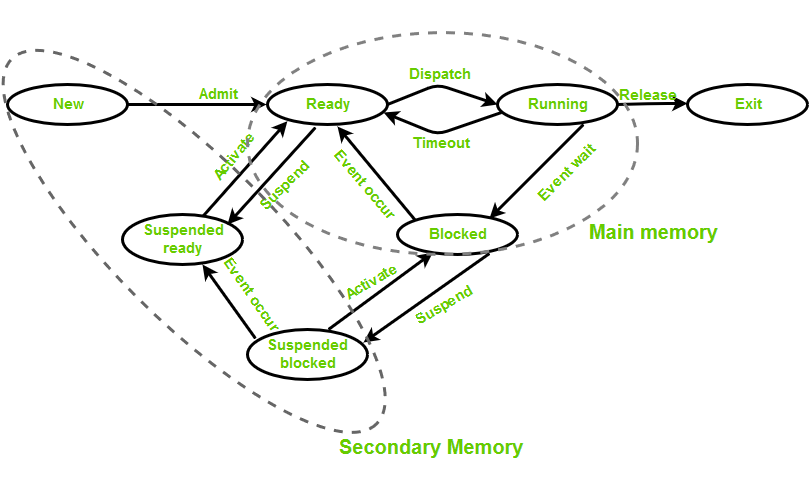
\includegraphics[scale = 0.565]{img/states_modified.png}
     \caption{General State Diagram of Transitions}
    \end{figure}
    \begin{figure}[Ht]
     \centering
     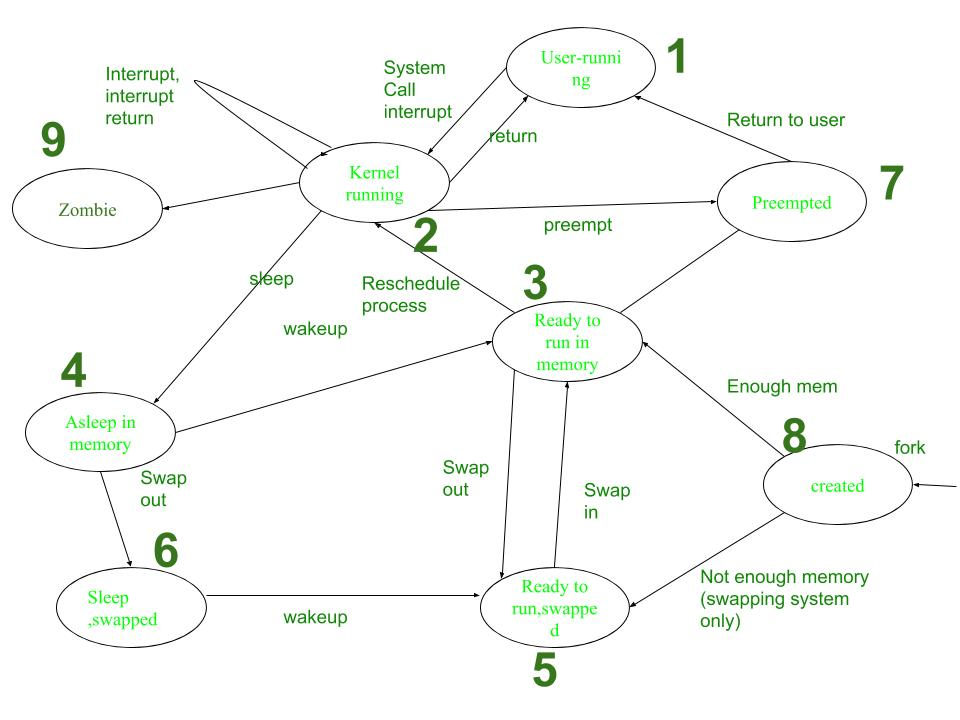
\includegraphics[scale = 0.35]{img/transitions.jpg}
     \caption{Transitions in a UNIX Process}
    \end{figure}

\section{Process API}
API is Application Programming Interface which is a collection of communication protocols and subroutines used by various programs to communicate between them. Briefly defined as functions available to write user programs.

API provided by OS is  a set of system calls which is a functional call into OS that runs at higher priority level of CPU. These are sensitive operations for example accessing hardware etc. Some system call may even cause process to be blocked and rescheduled.
\subsection{System Calls in Linux}
This a procedure that provides the interface between a process and the operating system. It is the way by which a computer program requests a service from the kernel of the operating system. Different operating systems execute different system calls.

In Linux, making a system call involves transferring control from unprivileged user mode to privileged kernel mode; the details of this transfer vary from architecture to architecture. The libraries take care of collecting the system-call arguments and, if necessary, arranging those arguments in the special form necessary to make the system call. \\
\textbf{Process Control}: \\
This system calls perform the task of process creation, process termination, etc. The Linux System calls under this are fork() , exit() , exec().
\subsubsection{Fork()}
\begin{itemize}
    \item A new process is created by making a copy of parent’s memory image
    \item The new process is added to OS process list and scheduled
    \item Parent and Child start execution just after fork and modify the memory data independently
\end{itemize}
    \begin{figure}[ht]
     \centering
     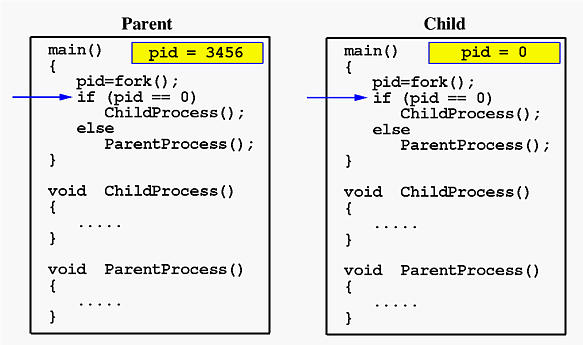
\includegraphics[scale = 0.565]{img/fork.jpg}
     \caption{The fork() system call}
    \end{figure}
\subsection{Exec()}
\begin{itemize}
    \item After fork, parent and child are running same code
    \item A process can run exec() to load another executable to its memory image
    \item Variants of exec() are used to pass commanline arguments to new executable
\end{itemize}
    \begin{figure}[ht]
     \centering
     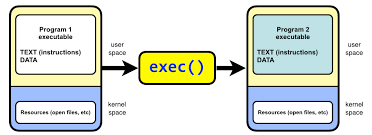
\includegraphics[scale = 0.8]{img/exec().png}
     \caption{The exec() system call}
    \end{figure}

\section{Mechanism of Process Execution}
\textbf{Process Execution}: \\
\begin{itemize}
    \item OS allocates memory and creates memory image
    \item Points CPU PC to current instruction
    \item After setup, OS is out of way and process executes directly on CPU
\end{itemize}
\textbf{OS Scheduler}: \\
\begin{itemize}
    \item The scheduler has 2 parts respectively named Policy and Mechanism
    \item Cooperative schedulers are polite and switch only if process is blocked
    \item non-cooperative schedulers can switch even when process is ready to continue where CPU generates periodic timer interrupts
    \item After interrupt the OS checks if current process has run long enough or not
\end{itemize}

\section{Scheduling Policies}
CPU Scheduling is a process that allows one process to use the CPU while another process is delayed (in standby) due to unavailability of any resources such as I / O etc, thus making full use of the CPU. The purpose of CPU Scheduling is to make the system more efficient, faster, and fairer.
\textbf{What are we optimizing?}: \\
\begin{itemize}
    \item maximize the utilization 
    \item minimize average time i.e time from process arrival to first scheduling
    \item minimize average response time
    \item fairness that all processes have same priority
    \item minimize overhead i.e run process long enough to reduce cost of context switch
\end{itemize}

Few policies include First-In-First-Out (FIFO), Shortest Job First (SJF), Shortest Time-to-Completion First (STCF), Round Robin (RR) etc. Each policy has its merits and demerits. \\
\textbf{Example}: Linux uses a Multi Level Feedback Queue (MLFQ)

\section{Inter Process Communication (IPC}
This is a mechanism provided by the operating system that allows processes to communicate with each other. This communication could involve a process letting another process know that some event has occurred or the transferring of data from one process to another.
\subsection{Shared Memory}
Processes can both access same region of memory via "shmget()" system call. By providing same key, 2 processes can get same segment of memory. They can read or write to memory to communicate.
\subsection{Signals}
A certain set of signals are supported by OS. Signals can be sent to a process by OS. There's a signal handler where every process has a default code to execute for each signal. Some signal handlers can be overridden to do other things also.
\subsection{Sockets}
Sockets can be used for two processes on same machine or different machines to communicate. TCP or UDP sockets are present across machines. Communication with sockets is done when processes open sockets and connect them to each other. Messages written into one socket can be read from another. The OS transfers data across socket buffers
\subsection{Pipes}
Pipe system call returns two file descriptions which are read and write handles. A pipe is a half-duplex communication. The data written in one file descriptor can be read through another.

There are two types of pipes \textbf{Regular Pipes} and \textbf{Named Pipes}. In regular pipes, parent and child share fd after fork where parent and child use respective ends of the pipe. In named pipes, two endpoints of a pipe can be in different processes. Pipe data buffered in OS buffers between write and read.

\section{Introduction to Virtual Memory}
Virtual Memory is a storage allocation scheme in which secondary memory can be addressed as though it were part of the main memory. The addresses a program may use to reference memory are distinguished from the addresses the memory system uses to identify physical storage sites, and program-generated addresses are translated automatically to the corresponding machine addresses. 

The size of virtual storage is limited by the addressing scheme of the computer system and the amount of secondary memory is available not by the actual number of the main storage locations.
Now multiple active processes timeshare CPU. We are using virtual memory because the real view of memory is very messed up.
\textbf{Goals of Virtualization}
\begin{itemize}
    \item Transparency: user programs should not be aware of the messy details
    \item Efficiency: minimize overhead and wastage in terms of memory space and access time
    \item Isolation and protection: a user process should not be able to access anything outside its address space
\end{itemize}
\subsection{Allocating Memory}
OS allocates a set of pages to the memory image of the process. Within the image static variables are allocated in the executable. Local variables of a function are on stack and Dynamic allocation is done with "malloc" on the heap

    \begin{figure}[ht]
     \centering
     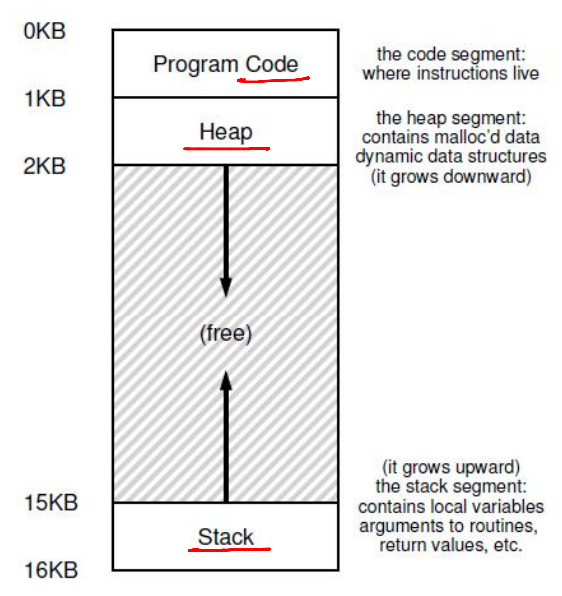
\includegraphics[scale = 0.6]{img/Address_Space.png}
     \caption{Address Space}
    \end{figure}
    
\section{Address Translation}
Virtual address space is setup by OS during process creation. A simplifies OS places entire memory image into one chunk. CPU provides the mode of execution in translation. ISA has instructions that set translation information. 

Hardware uses this information to perform translation on every memory access. This hardware generates faults and traps to OS when access is illegal.
\subsection{Role of OS in Translation}
\begin{itemize}
    \item OS maintains free list of memory
    \item Allocates space to process during creation and cleans up when done
    \item Maintains information of where space is allocated to each process in PCB
    \item Sets address translation information in hardware and updates this information upon context switch
\end{itemize}

\section{Paging}
Paging is a memory management scheme that eliminates the need for contiguous allocation of physical memory. This scheme permits the physical address space of a process to be non–contiguous.
\begin{itemize}
    \item Logical Address or Virtual Address : An address generated by the CPU
    \item Logical Address Space or Virtual Address Space: The set of all logical addresses generated by a program
    \item Physical Address : An address actually available on memory unit
    \item Physical Address Space : The set of all physical addresses corresponding to the logical addresses
\end{itemize}

    \begin{figure}[ht]
     \centering
     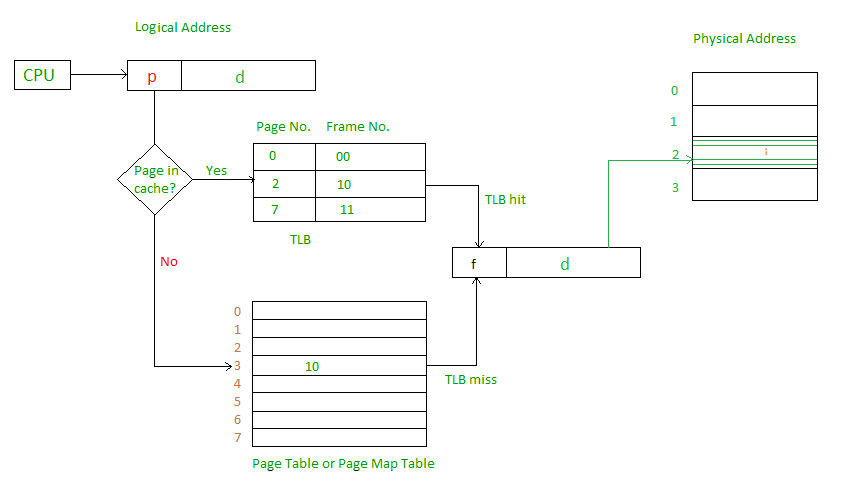
\includegraphics[scale = 0.45]{img/paging.jpg}
     \caption{Paging}
    \end{figure}


\section{Memory Allocation Algorithms}
In the operating system, the following are four common memory management techniques.Single contiguous allocation, Partitioned allocation, Paged memory management, Segmented memory management. 
Most of the operating systems (for example Windows and Linux) use Segmentation with Paging. A process is divided into segments and individual segments have pages.

\subsection{Variable sized allocation:}
Considering a simple implementation of "malloc", every allocated chunk has a header with info like size of chunk.
\subsection{Free List}
Free space is managed as a list. Pointer to the next free chunk is embedded within the free chunk. The library tracks the head of the list – Allocations happen from the head.
\subsection{Variable Size Allocation Strategies}
\begin{itemize}
    \item First fit: allocate first free chunk that is sufficient
    \item Best fit: allocate free chunk that is closest in size
    \item Worst fit: allocate free chunk that is farthest in size
\end{itemize}
\section{Threads and Concurrency}
A thread is a path of execution within a process. A process can contain multiple threads. A thread is also known as lightweight process. The idea is to achieve parallelism by dividing a process into multiple threads. 

For example, in a browser, multiple tabs can be different threads. MS Word uses multiple threads: one thread to format the text, another thread to process inputs, etc.

Concurrency is the execution of the multiple instruction sequences at the same time. It happens in the operating system when there are several process threads running in parallel. The running process threads always communicate with each other through shared memory or message passing.
    \begin{figure}[ht]
     \centering
     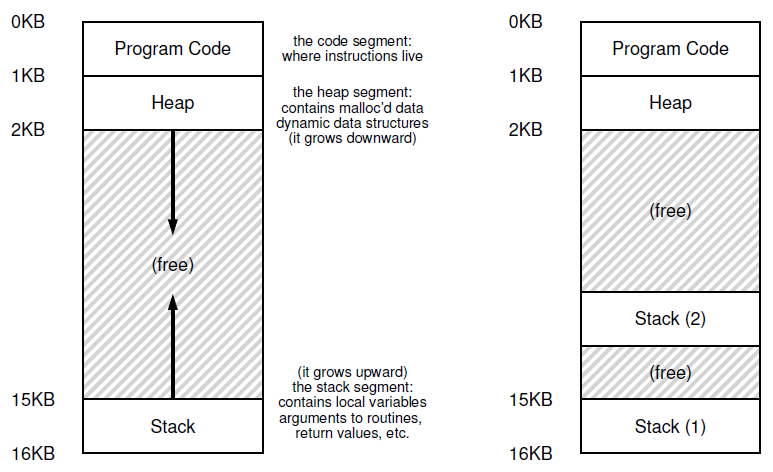
\includegraphics[scale = 0.5]{img/Threaded.png}
     \caption{Single-Threaded And Multi-Threaded Address Spaces}
    \end{figure}
\subsection{Single Threaded Process}
Single threaded processes contain the execution of instructions in a single sequence. In other words, one command is processes at a time. The opposite of single threaded processes are multithreaded processes. These processes allow the execution of multiple parts of a program at the same time. These are lightweight processes available within the process.
\subsection{Multi threaded process}
Multithreading is the ability of a program or an operating system to enable more than one user at a time without requiring multiple copies of the program running on the computer. Multithreading can also handle multiple requests from the same user.
\subsection{Threads}
A single process can effectively utilize multiple CPU cores which is known as Parallelism. Concurrency means running multiple threads/processes at the same time, even on single CPU core, by interleaving their executions.Parallelism means running multiple threads/processes in parallel over different CPU cores.
\subsection{Scheduling Threads}
Scheduling of threads involves two boundary scheduling:
\begin{itemize}
    \item Scheduling of user level threads (ULT) to kernel level threads (KLT) via lightweight process (LWP) by the application developer.
    \item Scheduling of user level threads (ULT) to kernel level threads (KLT) via lightweight process (LWP) by the application developer.
\end{itemize}
\section{Locks}
We use a special lock variable to protect shared variables. All threads accessing a critical section share a lock. One threads succeeds in locking – owner of lock. Other threads that try to lock cannot proceed further until lock is released by the owner.Pthreads library in Linux provides such locks.
\subsection{Building Locks}
Lock Implementation:
\begin{itemize}
    \item Mutual Exclusion and implemeting needs support from OS and hardware
    \item All threads should eventually get the lock, and no thread should starve
    \item Acquiring, releasing, and waiting for lock should not consume too many resources i.e low overhead
\end{itemize}
\subsection{Usage of Locks}
\begin{itemize}
    \item A lock should be acquired before accessing any variable or data structure that is shared between multiple threads of a process
    \item All shared kernel data structures must also be accessed only after locking
    \item Fine-grained allows more parallelism
    \item Multiple fine-grained locks may be harder to manage
\end{itemize}
\section{Condition Variables}
A condition variable (CV) is a queue that a thread can put itself into when waiting on some condition. Another thread that makes the condition true can signal the CV to wake up a waiting thread. Pthreads provides CV for user programs. Signal wakes up one thread, signal broadcast wakes up all waiting threads.
\section{Semaphores}
Synchronization primitive like condition variables. Semaphore is a variable with an underlying counter. There are two functions on a semaphore variable:
\begin{itemize}
    \item Up/post increments the counter
    \item Down/wait decrements the counter and blocks the calling thread if the resulting value is negative
    \item A semaphore with init value 1 acts as a simple lock
\end{itemize}
\section{Concurrency Bugs}
A concurrency bug is an (undesired) outcome that arises if two programs are run at the same time that does not show up if the two programs are run sequentially, one after the other. Common bugs in concurrent programs:
\begin{itemize}
    \item Bugs are non-deterministic and occur based on execution order of threads – very hard to debug
    \item Deadlocks: threads cannot execute any further and wait for each other
    \item Non-deadlock bugs: non deadlock but incorrect results when threads execute
\end{itemize}
\subsection{Deadlock Bugs}
In an operating system, a deadlock occurs when a process or thread enters a waiting state because a requested system resource is held by another waiting process, which in turn is waiting for another resource held by another waiting process.
    \begin{figure}[ht]
    \centering
    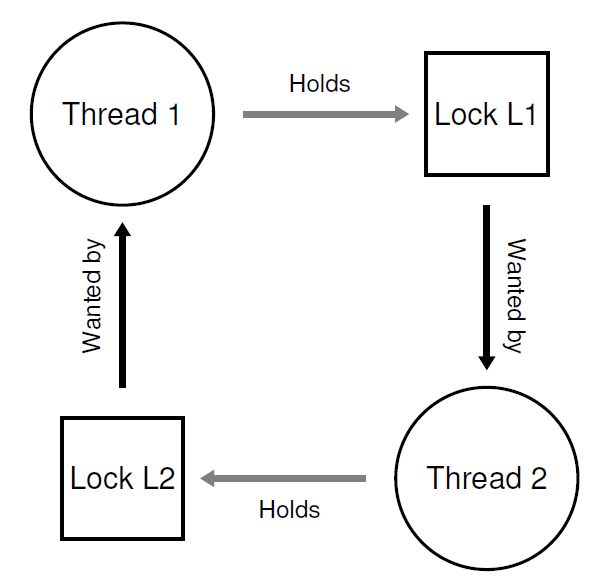
\includegraphics[scale = 0.3]{img/Deadblock.png}
    \caption{The Deadlock Dependency Graph}
    \end{figure}
\subsection{Non Deadlock Bugs}
\begin{itemize}
    \item Atomicity bugs: atomicity assumptions made by programmer are violated during execution
    \item Order-violation bugs: desired order of memory accesses is flipped during concurrent execution of concurrent threads
\end{itemize}
\section{Files and Directories}
\subsection{The File Abstraction}
\begin{itemize}
    \item File is a linear array of bytes that is stored persistently. It is identified with file name and a OS-level identifier. Inode number unique within the file system.
    \item Directory contains other subdirectories and files along with their inode numbers. These are stored like a file whose contents are filename-to-inode mappings
\end{itemize}
\subsection{Directory Tree}
By placing directories within other directories, users are able to build an arbitrary directory tree (or directory hierarchy), under which all files and directories are stored.
    \begin{figure}[ht]
    \centering
    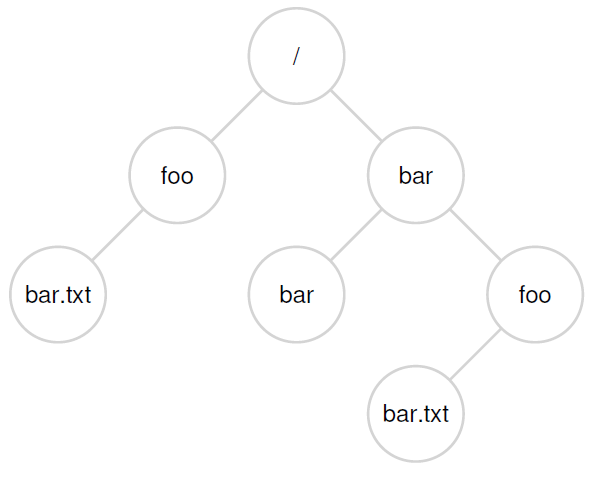
\includegraphics[scale =0.3]{img/DirectoryTree.png}
    \caption{An Example Directory Tree}
    \end{figure}
\subsection{Operations}
Operations on Files:
\begin{itemize}
    \item Creating a file and Opening a file
    \item Reading/writing files
    \item Close system call
    \item Seek and Sync
\end{itemize}
Operations on Directories are similar to as for files, and they can be accessed by create, open, read, close. 
\section{File System Implementation}
\subsection{File System}
\begin{itemize}
    \item An organization of files and directories on disk
    \item OS has one or more file systems
    \item Data structures to organize data and metadata on disk
    \item Implementation of system calls like open, read, write using the data structures
    \item Disks expose a set of blocks. System Calls translated into reads and writes on blocks
\end{itemize}
\pagebreak
\subsection{Inode Table}
    \begin{figure}[ht]
    \centering
    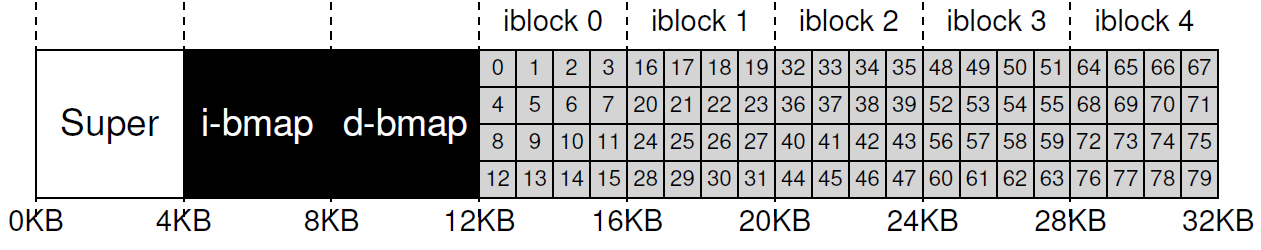
\includegraphics[scale = 0.3]{img/InodeTable.png}
    \caption{Inode Table}
    \end{figure}
Usually Inodes are stored in array. Inode number of file is index into this array. Inode stores file metadata like permissions, access time, etc and pointers of file data i.e disk block numbers.
\subsection{Inode Structure}
File data not stored contiguously on disk, need to track multiple block numbers of a file.
Inode tracking disk block numbers:
\begin{itemize}
    \item Direct pointers: numbers of first few blocks are stored in inode itself (suffices for small files)
    \item Indirect block: for larger files, inode stores number of indirect block, which has block numbers of file data.
    \item In the same way double and triple indirect blocks are tracked.
\end{itemize}
\subsection{File Allocation Table (FAT)}
This is a alternate way to track file blocks. FAT stores next block pointer for each block. FAT has 1 entry per disk block. Entry has number of next file block or null. Pointer to first block is stored in inode.
\subsection{Directory Structure}
\begin{itemize}
    \item Directory stores records mapping filename to inode number
    \item Linked list of records, or more complex structures like hash tables, binary search trees etc.
    \item Directory is a special type of file and has inode and data blocks
\end{itemize}
\subsection{Free Space Management}
We track free blocks using Bitmaps, Free list and other complex structures.
\begin{itemize}
    \item Bitmaps: For inodes and data blocks, we store 1 bit per block to indicate if free or not
    \item Free List: Super block stores pointer to first free block, a free block stores address of next block on list
\end{itemize}
\subsection{Virtual File System}
A virtual file system (VFS) is programming that forms an interface between an operating system's kernel and a more concrete file system. The VFS serves as an abstraction layer that gives applications access to different types of file systems and local and network storage devices
\begin{itemize}
    \item File systems differ in implementations of data structures (e.g., organization of file records in directory)
    \item Linux supports virtual file system (VFS) abstraction
    \item VFS looks at a file system as objects (files, directories, inodes, superblock) and operations on these objects (e.g., lookup filename in directory)
    \item System call logic is written on VFS objects
    \item To develop a new file system, simply implement functions on VFS objects and provide pointers to these functions to kernel
    \item Syscall implementation does not have to change with file system implementation details
\end{itemize}
\subsection{Disk Buffer Cache}
 Disk buffer is the embedded memory in a hard disk drive (HDD) acting as a buffer between the rest of the computer and the physical hard disk platter that is used for storage. It is physically distinct from and is used differently from the page cache typically kept by the operating system in the computer's main memory.
 It is controlled by the microcontroller in the hard disk drive, and the page cache is controlled by the computer to which that disk is attached.
 \begin{itemize}
     \item Results of recently fetched disk blocks are cached
     \item File system issues block read/write requests to block numbers via buffer cache
     \begin{itemize}
         \item If block in cache, served from cache, no disk I/O
         \item If cache miss, block fetched to cache and returned to file system
     \end{itemize}
     \item Writes are applied to cache block first
     \begin{itemize}
         \item Synchronous/write-through cache writes to disk immediately
         \item Asynchronous/write-back cache stores dirty block in memory and writes back after a delay
     \end{itemize}
     \item Unified page cache in OS where free pages allocated to both processes and cache from common pool
 \end{itemize}
 Benefits of disk buffer cache are that there is improved performance due to reduced disk I/O and there is single copy of block in memory which gives consistency across processes
 


\end{document}
